\section{Konzeptionelles Datenmodell}\label{sec:konzeptionelles-datenmodell}

Das folgende Klassendiagramm ist als \texttt{svg}-Datei im Rootverzeichnis des Repositorys gespeichert (\texttt{./class-diagram.svg}).
Ebenso befindet sich dort ein zweites Klassendiagramm, das ebenfalls zusätzlich Interfaces, Exception- und Service-Klassen beinhaltet.

\begin{figure}[H]
    \centering
    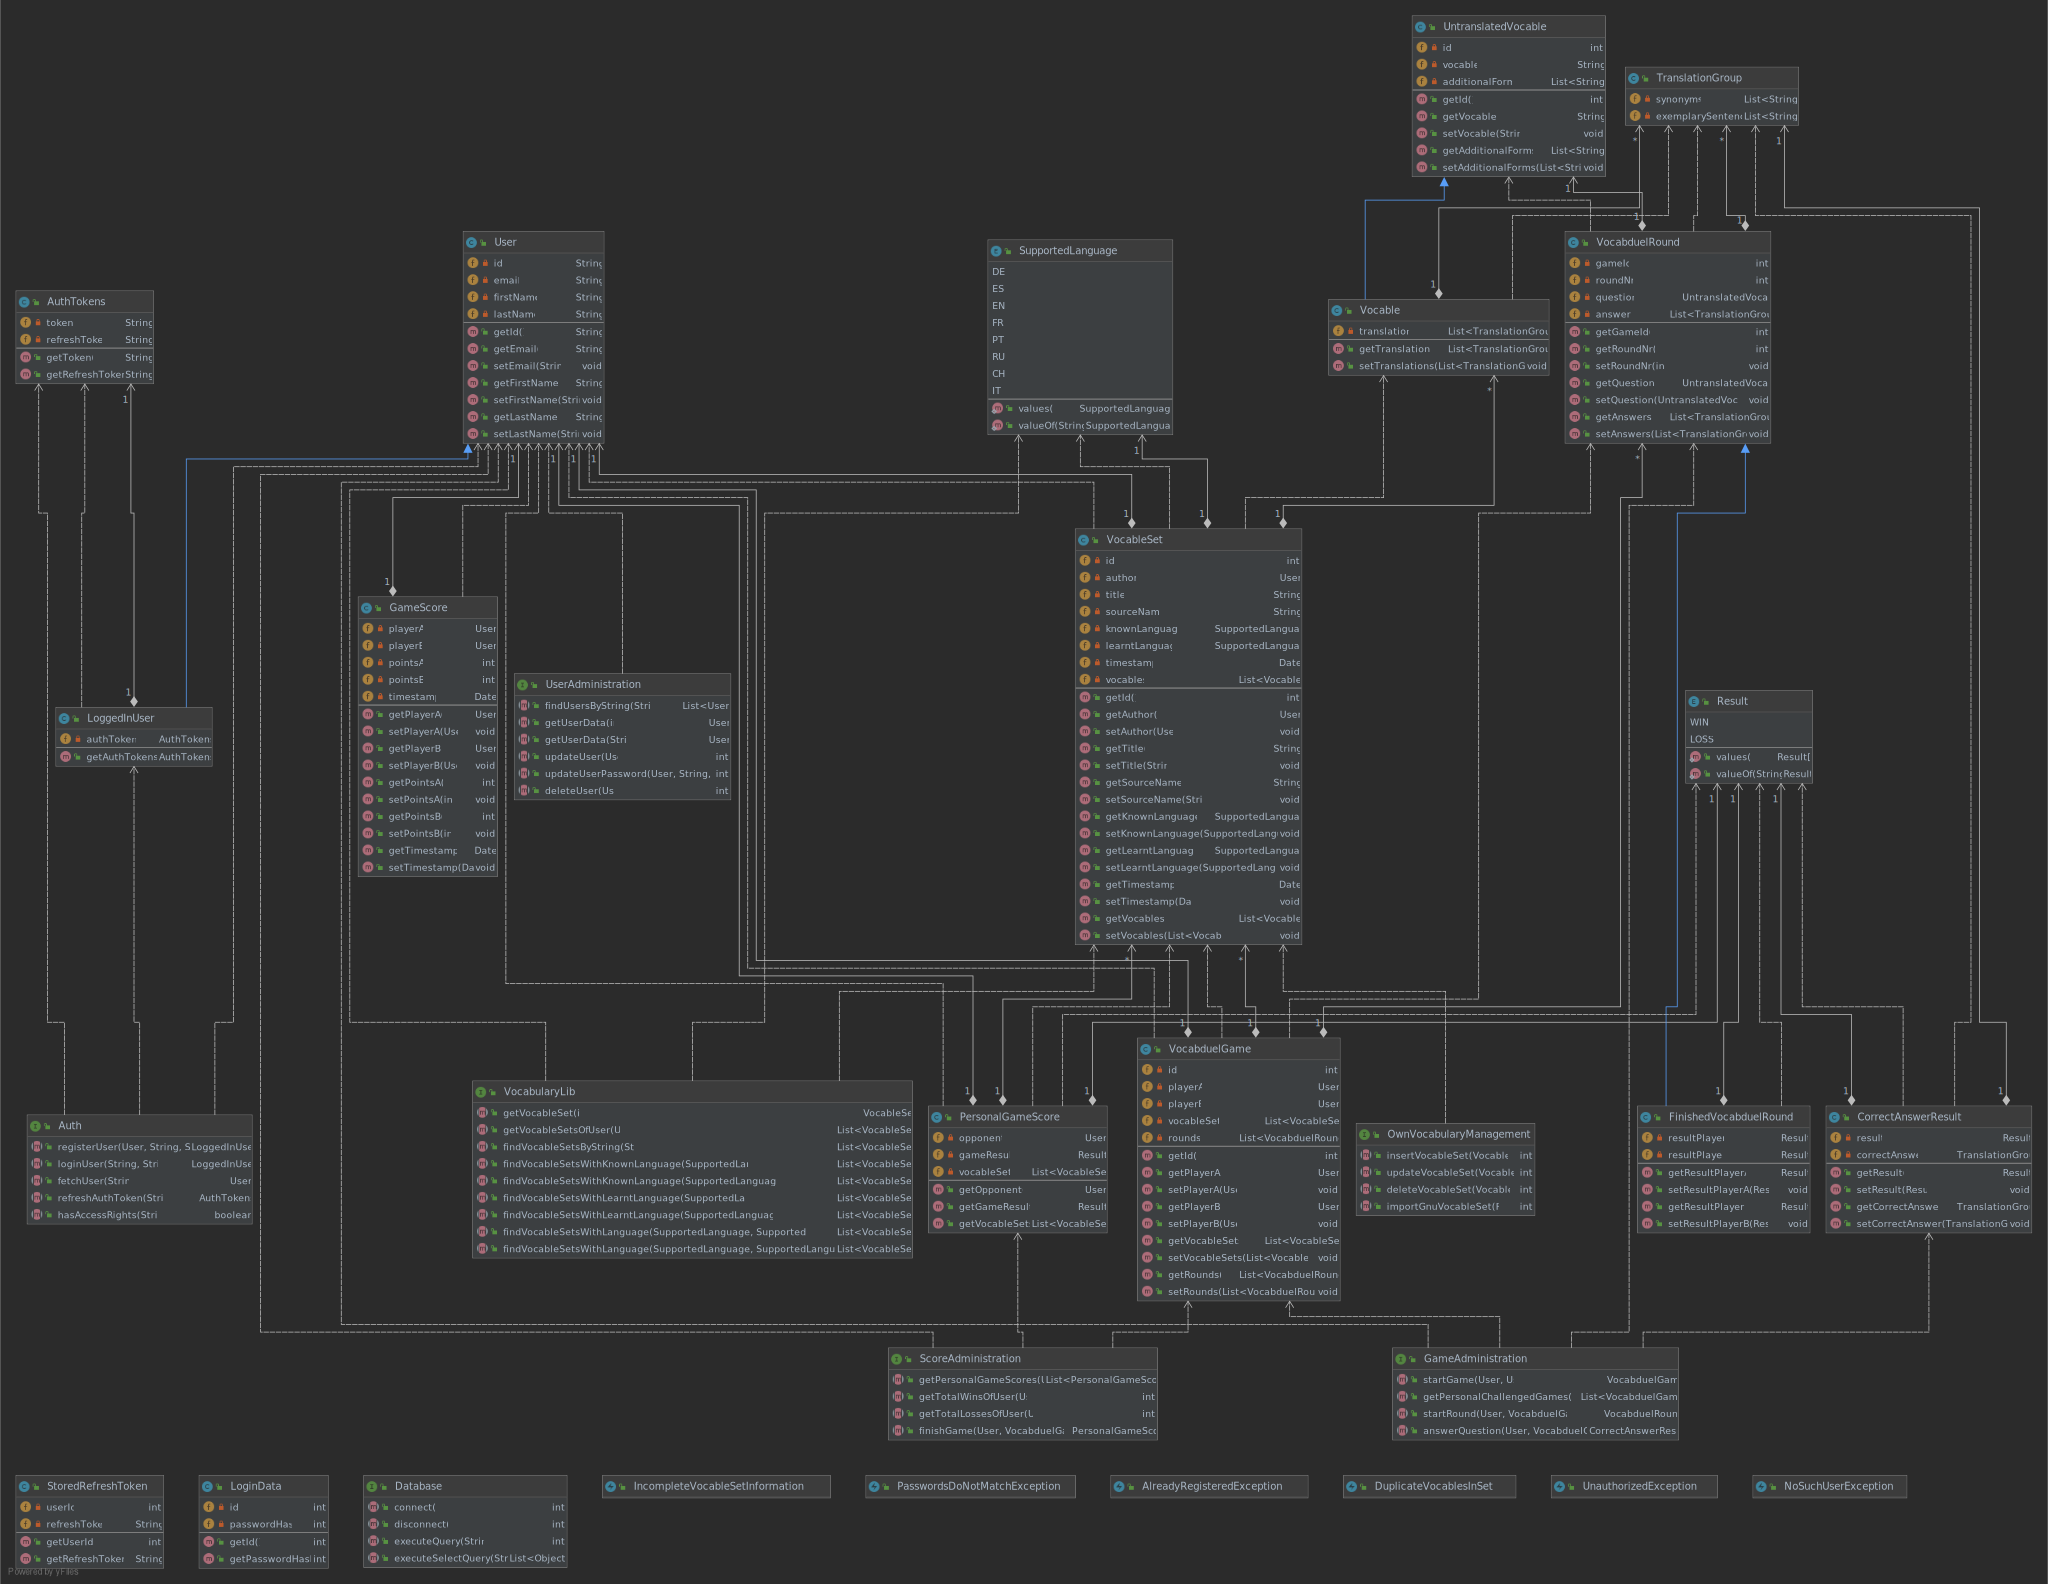
\includegraphics[width=1\textwidth]{class-diagram}
    \caption[]{Klassendiagramm}
    \label{fig:classes}
\end{figure}

Im Folgenden wird das konzeptionelle Datenmodell beschrieben, welches auch tatsächlich in ein physikalisches Datenmodell überführt wurde.

Die Entität LoginData erbt vom User Username, Email, Vor- und Zuname und speichert validierte, verschlüsselte Passwörter, die der User zum Login benötigt.
Ist der User eingeloggt, stellen die StoredRefreshToken sicher, dass der User mit gültigen Token versorgt wird, was etwa
einer gültigen Web-Session des Users auf einer Web-Applikation gleich kommt.
User mit StoredRefreshToken werden im LoggedInUser festgehalten, was aber kein Bestandteil des physikalischen Datenmodells ist.

Zur Verwaltung von Vokabellisten werden Begriffe in Synonyme und zusätzliche Informationen (additionalInfo) getrennt und in TranslationGroups einander zugeordnet.
Mit dem Erhalt einer zusätzlichen Id wird aus dem Begriff eine UntranslatedVocable.
Eine Vokabel ist schließlich die Zuordnung einer UntranslatedVocable mit anderen Begriffen.
Da UntranslatedVocable und Vocable eine gemeinsame Datenbank Tabelle darstellen,
wird zusätzlich die Spalte Datentyp (DTYPE) gestellt, um zwischen beiden Entitäten zu unterscheiden.
Beispielsatzbausteine in Lern- (UntranslatedVocable) oder Wissenssprache (Vocable) können auch in dieser Tabelle gespeichert werden.
Aus mehreren Vokabeln, Autor-Angabe, Titel und createdTimestamp wird eine Vokabelliste und aus mehreren Vokabellisten und Titel
wird eine VokabelUnit.

VokabelUnits werden mit Lern- und Wissenssprache zu einem LanguageSet.
Um mit Vokabellisten spielen zu können, werden die Spiele in RunningVocabduelGames mit Lern- und Wissenssprache sowie zwei User- und einer Vokabellist-Zuordnungen gespeichert.
Beim Spiel ist so festgehalten, welche Vokabelliste für dieses Spiel genutzt wird. Die Duell-Runden werden einzelnen Translationgroups zugeordnet, um einen Begriff zum Übersetzen zu haben.
Die möglichen Antwortmöglichkeiten zur Runde werden nicht in der Datenbank gespeichert, ebensowenig, wie die richtige Übersetzung für die Runde lautet.
Da wir die richtige Übersetzung bereits aus der Vokabel erhalten, wird für die fertig gespielte Runde nur das Ergebnis "WIN" oder "LOSS" gespeichert.
Noch laufende Runden und fertig gespielte Runden werden in derselben physikalischen Tabelle gespeichert und sind am Eintrag des Rundenergebnisses zu erkennen.
Wurden alle Runden eines Spiels gespielt, so wird ein fertig gespieltes Spiel gespeichert. Hier wird die erreichte Endpunktzahl zum Spiel von jedem Teilnehmer hinterlegt.
Ob ein Spieler damit gewonnen, verloren oder unentschieden gespielt hat, wird nicht in der Datenbank gespeichert, sondern auf dem Server ermittelt.
